\subsection{DOP 10 Классификация  языков,  определяемых  конечными  автоматами,  регулярными  выражениями  и праволинейными грамматиками. Эквивалентность и минимизация конечных автоматов.}

\textbf{Грамматики и регулярные множества и выражения}
\begin{itemize}
    \item \textbf{Грамматика} --- это четверка $G = (N, T, P, S)$, где $N$ --- \textbf{алфавит нетерминальных символов}, $T$ --- \textbf{алфавит терминальных символов}, $N \cap T = \varnothing$, $P$ --- \textbf{конечное множество правил} вида $\alpha \rightarrow \beta$, где $\alpha \in (N \cup T)^+$ (хотя бы 1)$,~\beta \in (N \cup T)^\ast,~S \in N$ --- \textbf{начальный знак} или аксиома грамматики.
    \item \textbf{Отношение выводимости} $\Rightarrow$ --- если $\gamma \rightarrow \delta \in P$, то $\alpha \gamma \beta \Rightarrow \alpha \delta \beta$, $\forall \alpha,~\beta \in (N \cup T)^\ast$.
    \item \textbf{Сентенциальная форма} грамматики $G$ --- цепочка, выводимая из ее начального символа.
    \item \textbf{Языком}, порождаемым грамматикой $G$ $(L(G))$ называется множество всех её терминальных сентенциальных форм $L(G) = \{ w |w \in T^\ast , S \Rightarrow^{\ast}_G w\}$.
    \item Грамматики \textbf{эквивалентны}, если они порождают один и тот же язык.
    \item \textbf{Классификация грамматик по Хомскому:}
    \begin{description}
        \item[Тип 0] Любая порождающая грамматика.
        \item[Тип 1] (Неукорачивающая или контекстно-зависимая грамматика) Если каждое правило кроме $S \rightarrow e$ имеет вид $\alpha \rightarrow \beta$, где $|\alpha| \leqslant |\beta|$, и в том случае, когда $S \rightarrow e \in P$, $S$ не встречается в правых частях правил.
        \item[Тип 2] (Контекстно-свободная грамматика.) Если каждое правило имеет вид $A \rightarrow \beta$, где $A \in N,~\beta \in (N \cup T)^\ast$.
        \item[Тип 3] (Регулярная праволинейная (или леволинейная) грамматика.) Каждое правило имеет вид либо $A \rightarrow xB$, либо $A \rightarrow x$, где $A,~B \in N,~x \in T^\ast$. (для леволинейных поменять $xB$ на $Bx$.)
    \end{description}
    \item \textbf{Типом языка} называется максимальный тип грамматики, порождающей этот язык.
    \item \textbf{Регулярное множество} определяется рекурсивно:
    \begin{enumerate}
        \item $\varnothing$ --- регулярное множество в алфавите $T$.
        \item $\{e\}$ --- регулярное множество в $T$, где $e$ --- пустая цепочка.
        \item $\{a\}$ --- регулярное множество в $T$ для каждого $a \in T$.
        \item Если $P$ и $Q$ --- регулярные множества в $T$, то регулярными являются $P \cup Q$ (объединение), $P Q$ (конкатенация), $P^\ast$ (итерация).
        \item Ничто другое не является регулярным множеством.
    \end{enumerate}
    \item \textbf{Регулярное выражение} определяется рекурсивно:
    \begin{enumerate}
        \item $\varnothing$ --- регулярное выражение, обозначающее рег. множество $\varnothing$.
        \item $e$ --- регулярное выражение, определяющее рег. множество $\{e\}$.
        \item $a$ --- регулярное выражение, определяющее рег. множество $\{a\}$.
        \item Если $p$ и $q$ --- регулярные выражения, то регулярными являются $(p | q)$ (обозначает множество $P \cup Q$), $p q$ (обозначает множество $P Q$), $p^\ast$ (обозначает множество $P^\ast$).
        \item Ничто другое не является регулярным выражением.
    \end{enumerate}
\end{itemize}

\textbf{Конечные автоматы}

Для распознавания регулярных множеств служат конечные автоматы.
\begin{itemize}
    \item \textbf{Недетерминированный КА} --- пятёрка $M = (Q, T, D, q_0, F)$ где $Q$ --- \textbf{конечное множество состояний}, $T$ --- \textbf{входной алфавит}, $D$ --- \textbf{функция переходов}, отображающая множество $Q \times (T \cup \{e\})$ во множество подмножеств $Q$, $q_0 \in Q$ --- \textbf{начальное состояние}, $F \subseteq Q$ --- \textbf{множество заключительных состояний}.
    \item \textbf{Детерминированный КА} --- НКА, в котором $D(q, e) = \varnothing$ для любого $q \in Q$ и $D(q, a)$ содержит не более 1 элемента для любых $q \in Q$ и $a \in T$.
    \item \textbf{Теорема 1.} 
    Язык, допускаемый ДКА, --- множество всех его допустимых цепочек --- является регулярным множеством.
    % \item Праволинейная грамматика $G = (N, T, P, S)$ называется \textbf{регулярной}, если каждое правило, кроме $S \rightarrow e$, имеет вид либо $A \rightarrow aB$, либо $A \rightarrow a$, где $A,~B \in N$, $a \in T$ и в том случае, когда $S \rightarrow e \in P$, $S$ не встречается в правых частях правил. 
    % Для всякой праволинейной грамматики существует регулярная грамматика такая, что порождаемые ими языки равны.
    \item \textbf{Теорема 2.} 
    Пусть $G = (N, T, P, S)$ --- праволинейная. 
    Тогда существует НКА $M = (Q, T, D, q_0, F)$, для которого $L(M) = L(G)$.
    \item \textbf{Теорема 3.} 
    Для каждого НКА $M$ существует праволинейная грамматика $G$ такая, что $L(M) = L(G)$. 
    По НКА можно построить эквивалентный ему ДКА. 
    По ДКА можно построить эквивалентный ДКА с минимальным числом состояний.
\end{itemize}


\textbf{Состояние $s$ конечного автомата $M$ эквивалентно} состоянию $t$ конечного автомата $N$ тогда и только тогда, когда автомат $M$, начав работу в состоянии $s$ будет допускать в точности те же цепочки, что и автомат $N$, начавший работу в состоянии $t$.

\textbf{Два автомата $M_1$ и $M_2$ называются эквивалентными}, если их входные алфавиты совпадают и для каждого состояния $M_1$ существует эквивалентное ему состояние $M_2$.

\textbf{Алгоритм минимизации}:
\begin{enumerate}
    \item Удаляем все недостижимые состояния и те, из которых нет пути в конечное состояние.
    \item Разбиваем исходное множество состояний на два, первое из которых состоит из всех конечных состояний, а второе --- из всех остальных: $\{F\},~\{Q \setminus F\}$.
    \item Если элементы одного множества при переходе по одному символу попадают в разные множества, то разбиваем исходное множество так, чтобы в одном множестве оказались только те состояния, которые переходят в состояния одного множества.
    Например пусть есть множества $\{s_1,s_2,s_3,s_4\},\{s_5,s_6\}$ и переходы $s_1 \xrightarrow{a} s_1$, $s_2 \xrightarrow{a} s_1$, $s_3 \xrightarrow{a} s_5$, $s_4 \xrightarrow{a} s_6$.
    Тогда новые множества будут иметь следующий вид: $\{s_1,s_2\},~\{s_3,s_4\},~\{s_5,s_6\}$.
    \item Продолжаем разбиение до тех пор, пока это возможно.
    \item Каждое множество состояний старого автомата заменяем на одно состояние нового.
\end{enumerate}

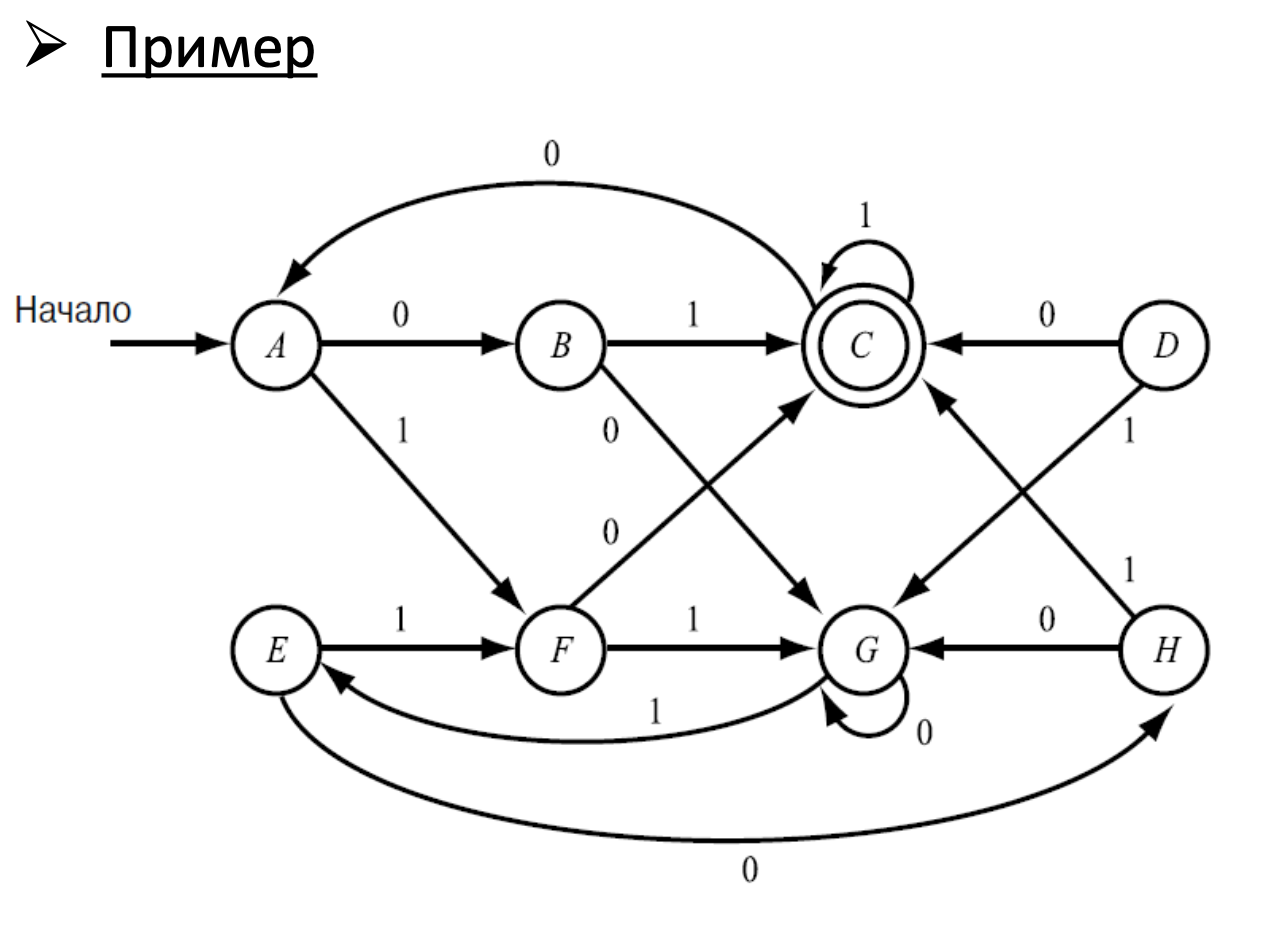
\includegraphics[width=0.24\textwidth]{pics/equivalence1.png}
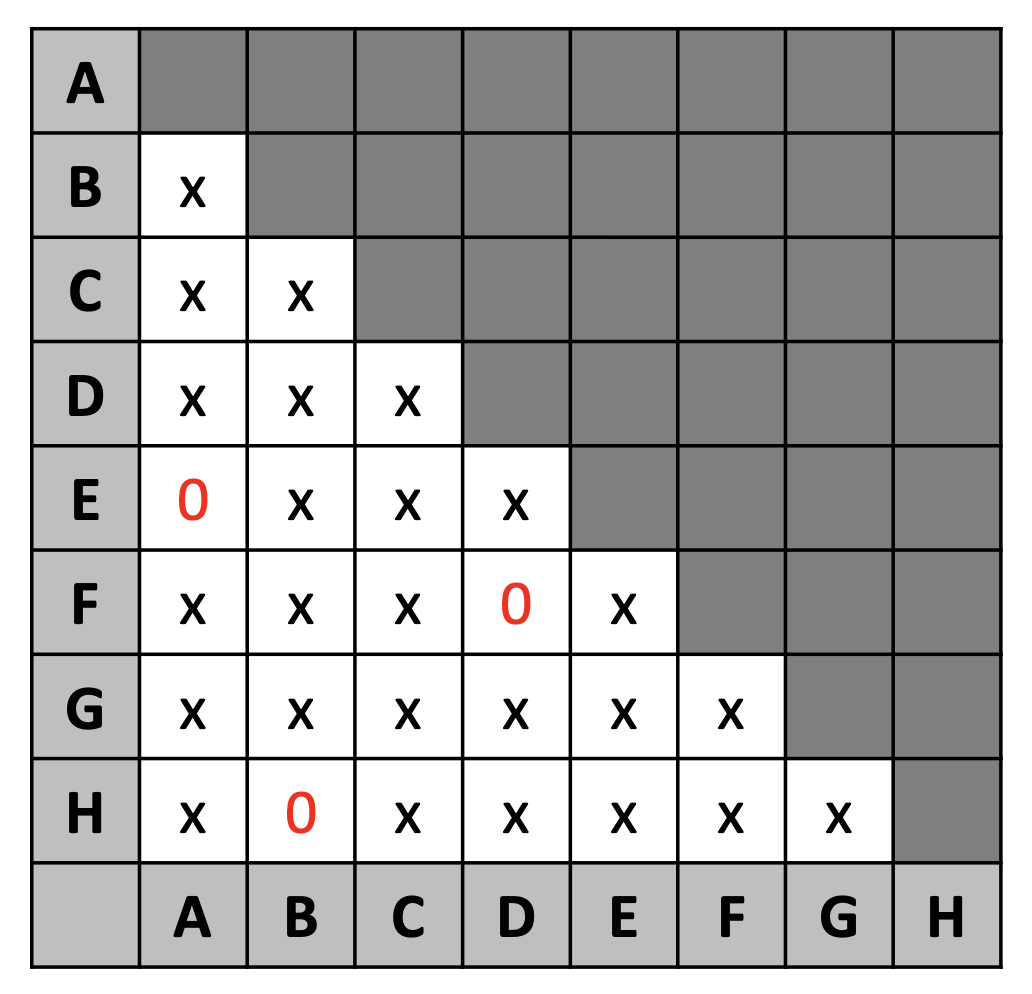
\includegraphics[width=0.17\textwidth]{pics/equivalence2.png}

Там где крестик - состояния неэквивалентны. Перебираем все возможные переходы из каждого состояния. В данном случае из каждого состояния по 0 и 1. Если два состояния переходят по одному символу в разные состояния, то ставится крестик (они уже неэквивалентны)

    


% -------- source --------
\bigbreak
[\cite[page 25-37]{ignatiev4}]